%  LaTeX support: latex@mdpi.com 
%  For support, please attach all files needed for compiling as well as the log file, and specify your operating system, LaTeX version, and LaTeX editor.

%=================================================================
\documentclass[mathematics,article,submit,pdftex,moreauthors]{Definitions/mdpi} 
% For posting an early version of this manuscript as a preprint, you may use "preprints" as the journal and change "submit" to "accept". The document class line would be, e.g., \documentclass[preprints,article,accept,moreauthors,pdftex]{mdpi}. This is especially recommended for submission to arXiv, where line numbers should be removed before posting. For preprints.org, the editorial staff will make this change immediately prior to posting.

%--------------------
% Class Options:
%--------------------
%----------
% journal
%----------
% Choose between the following MDPI journals:
% acoustics, actuators, addictions, admsci, adolescents, aerospace, agriculture, agriengineering, agronomy, ai, algorithms, allergies, alloys, analytica, animals, antibiotics, antibodies, antioxidants, applbiosci, appliedchem, appliedmath, applmech, applmicrobiol, applnano, applsci, aquacj, architecture, arts, asc, asi, astronomy, atmosphere, atoms, audiolres, automation, axioms, bacteria, batteries, bdcc, behavsci, beverages, biochem, bioengineering, biologics, biology, biomass, biomechanics, biomed, biomedicines, biomedinformatics, biomimetics, biomolecules, biophysica, biosensors, biotech, birds, bloods, blsf, brainsci, breath, buildings, businesses, cancers, carbon, cardiogenetics, catalysts, cells, ceramics, challenges, chemengineering, chemistry, chemosensors, chemproc, children, chips, cimb, civileng, cleantechnol, climate, clinpract, clockssleep, cmd, coasts, coatings, colloids, colorants, commodities, compounds, computation, computers, condensedmatter, conservation, constrmater, cosmetics, covid, crops, cryptography, crystals, csmf, ctn, curroncol, currophthalmol, cyber, dairy, data, dentistry, dermato, dermatopathology, designs, diabetology, diagnostics, dietetics, digital, disabilities, diseases, diversity, dna, drones, dynamics, earth, ebj, ecologies, econometrics, economies, education, ejihpe, electricity, electrochem, electronicmat, electronics, encyclopedia, endocrines, energies, eng, engproc, ent, entomology, entropy, environments, environsciproc, epidemiologia, epigenomes, est, fermentation, fibers, fintech, fire, fishes, fluids, foods, forecasting, forensicsci, forests, foundations, fractalfract, fuels, futureinternet, futureparasites, futurepharmacol, futurephys, futuretransp, galaxies, games, gases, gastroent, gastrointestdisord, gels, genealogy, genes, geographies, geohazards, geomatics, geosciences, geotechnics, geriatrics, hazardousmatters, healthcare, hearts, hemato, heritage, highthroughput, histories, horticulturae, humanities, humans, hydrobiology, hydrogen, hydrology, hygiene, idr, ijerph, ijfs, ijgi, ijms, ijns, ijtm, ijtpp, immuno, informatics, information, infrastructures, inorganics, insects, instruments, inventions, iot, j, jal, jcdd, jcm, jcp, jcs, jdb, jeta, jfb, jfmk, jimaging, jintelligence, jlpea, jmmp, jmp, jmse, jne, jnt, jof, joitmc, jor, journalmedia, jox, jpm, jrfm, jsan, jtaer, jzbg, kidney, kidneydial, knowledge, land, languages, laws, life, liquids, literature, livers, logics, logistics, lubricants, lymphatics, machines, macromol, magnetism, magnetochemistry, make, marinedrugs, materials, materproc, mathematics, mca, measurements, medicina, medicines, medsci, membranes, merits, metabolites, metals, meteorology, methane, metrology, micro, microarrays, microbiolres, micromachines, microorganisms, microplastics, minerals, mining, modelling, molbank, molecules, mps, msf, mti, muscles, nanoenergyadv, nanomanufacturing, nanomaterials, ncrna, network, neuroglia, neurolint, neurosci, nitrogen, notspecified, nri, nursrep, nutraceuticals, nutrients, obesities, oceans, ohbm, onco, oncopathology, optics, oral, organics, organoids, osteology, oxygen, parasites, parasitologia, particles, pathogens, pathophysiology, pediatrrep, pharmaceuticals, pharmaceutics, pharmacoepidemiology, pharmacy, philosophies, photochem, photonics, phycology, physchem, physics, physiologia, plants, plasma, pollutants, polymers, polysaccharides, poultry, powders, preprints, proceedings, processes, prosthesis, proteomes, psf, psych, psychiatryint, psychoactives, publications, quantumrep, quaternary, qubs, radiation, reactions, recycling, regeneration, religions, remotesensing, reports, reprodmed, resources, rheumato, risks, robotics, ruminants, safety, sci, scipharm, seeds, sensors, separations, sexes, signals, sinusitis, skins, smartcities, sna, societies, socsci, software, soilsystems, solar, solids, sports, standards, stats, stresses, surfaces, surgeries, suschem, sustainability, symmetry, synbio, systems, taxonomy, technologies, telecom, test, textiles, thalassrep, thermo, tomography, tourismhosp, toxics, toxins, transplantology, transportation, traumacare, traumas, tropicalmed, universe, urbansci, uro, vaccines, vehicles, venereology, vetsci, vibration, viruses, vision, waste, water, wem, wevj, wind, women, world, youth, zoonoticdis 

%---------
% article
%---------
% The default type of manuscript is "article", but can be replaced by: 
% abstract, addendum, article, book, bookreview, briefreport, casereport, comment, commentary, communication, conferenceproceedings, correction, conferencereport, entry, expressionofconcern, extendedabstract, datadescriptor, editorial, essay, erratum, hypothesis, interestingimage, obituary, opinion, projectreport, reply, retraction, review, perspective, protocol, shortnote, studyprotocol, systematicreview, supfile, technicalnote, viewpoint, guidelines, registeredreport, tutorial
% supfile = supplementary materials

%----------
% submit
%----------
% The class option "submit" will be changed to "accept" by the Editorial Office when the paper is accepted. This will only make changes to the frontpage (e.g., the logo of the journal will get visible), the headings, and the copyright information. Also, line numbering will be removed. Journal info and pagination for accepted papers will also be assigned by the Editorial Office.

%------------------
% moreauthors
%------------------
% If there is only one author the class option oneauthor should be used. Otherwise use the class option moreauthors.

%---------
% pdftex
%---------
% The option pdftex is for use with pdfLaTeX. If eps figures are used, remove the option pdftex and use LaTeX and dvi2pdf.

%=================================================================
% MDPI internal commands
\firstpage{1} 
\makeatletter 
\setcounter{page}{\@firstpage} 
\makeatother
\pubvolume{1}
\issuenum{1}
\articlenumber{0}
\pubyear{2022}
\copyrightyear{2022}
%\externaleditor{Academic Editor: Firstname Lastname}
\datereceived{} 
%\daterevised{} % Only for the journal Acoustics
\dateaccepted{} 
\datepublished{} 
%\datecorrected{} % Corrected papers include a "Corrected: XXX" date in the original paper.
%\dateretracted{} % Corrected papers include a "Retracted: XXX" date in the original paper.
\hreflink{https://doi.org/} % If needed use \linebreak
%\doinum{}
%------------------------------------------------------------------
% The following line should be uncommented if the LaTeX file is uploaded to arXiv.org
%\pdfoutput=1

%=================================================================
% Add packages and commands here. The following packages are loaded in our class file: fontenc, inputenc, calc, indentfirst, fancyhdr, graphicx, epstopdf, lastpage, ifthen, lineno, float, amsmath, setspace, enumitem, mathpazo, booktabs, titlesec, etoolbox, tabto, xcolor, soul, multirow, microtype, tikz, totcount, changepage, attrib, upgreek, cleveref, amsthm, hyphenat, natbib, hyperref, footmisc, url, geometry, newfloat, caption

%%% ДЛЯ РУССКОГО ТЕКСТА закомментировать потом!
\usepackage{inputenc}
\usepackage[T2A,T1]{fontenc}
\usepackage[english,russian]{babel}
\usepackage{cmap}
%%%


%=================================================================
%% Please use the following mathematics environments: Theorem, Lemma, Corollary, Proposition, Characterization, Property, Problem, Example, ExamplesandDefinitions, Hypothesis, Remark, Definition, Notation, Assumption
%% For proofs, please use the proof environment (the amsthm package is loaded by the MDPI class).

%=================================================================
% Full title of the paper (Capitalized)
\Title{Using the ... Algorithm to Detect Kinetic Parameters of Catalytic Isomerization of the Pentane-Hexane Fraction}
% Дежурное название: Использование ...алгоритма для определения кинетических параметров процесса каталитической изомеризации пентан-гексановой фракции


% MDPI internal command: Title for citation in the left column
\TitleCitation{Title}

% Author Orchid ID: enter ID or remove command
\newcommand{\orcidauthorA}{0000-0001-5273-2471} % Add \orcidA{} behind the author's name
\newcommand{\orcidauthorB}{0000-0002-8736-0652} % Add \orcidB{} behind the author's name
\newcommand{\orcidauthorC}{0000-0003-4219-4870} 

% Authors, for the paper (add full first names)
\Author{Konstantin Barkalov $^{1}$\orcidA{}, Irek Gubaydullin $^{2,3}$, Ilya Lebedev $^{1}$\orcidB{}, Roza Faskhutdinova $^{2,3}$ and Leniza Enikeeva $^{3,4,}$*\orcidC{}}

%\longauthorlist{yes}

% MDPI internal command: Authors, for metadata in PDF
\AuthorNames{Konstantin Barkalov, Irek Gubaydullin, Ilya Lebedev, Roza Faskhutdinova and Leniza Enikeeva}

% MDPI internal command: Authors, for citation in the left column
\AuthorCitation{Barkalov, B.; Gubaydullin, I.; Lebedev, I.; Faskhutdinova, R.; Enikeeva, L.}
% If this is a Chicago style journal: Lastname, Firstname, Firstname Lastname, and Firstname Lastname.

\address{%
$^{1}$ \quad Lobachevsky State University of Nizhny Novgorod, Nizhny Novgorod, Russia; konstantin.barkalov@itmm.unn.ru\\
$^{2}$ \quad Institute of Petrochemistry and Catalysis – Subdivision of the Ufa Federal Research Centre of RAS, Ufa, Russia; irekmars@mail.ru \\
$^{3}$ \quad Ufa State Petroleum Technological University, Ufa, Russia; roza\_fask@mail.ru\\
$^{4}$ \quad Novosibirsk State University, Novosibirsk, Russia; leniza.enikeeva@yandex.ru
}

% Contact information of the corresponding author
\corres{Correspondence: leniza.enikeeva@yandex.ru (E.L.); konstantin.barkalov@itmm.unn.ru (B.K.) }

% Current address and/or shared authorship
%\firstnote{Current address: Affiliation 3.} 
%\secondnote{These authors contributed equally to this work.}
% The commands \thirdnote{} till \eighthnote{} are available for further notes

%\simplesumm{} % Simple summary

%\conference{} % An extended version of a conference paper

% Abstract (Do not insert blank lines, i.e. \\) 
\abstract{A single paragraph of about 200 words maximum. For research articles, abstracts should give a pertinent overview of the work. We strongly encourage authors to use the following style of structured abstracts, but without headings: (1) Background: place the question addressed in a broad context and highlight the purpose of the study; (2) Methods: describe briefly the main methods or treatments applied; (3) Results: summarize the article's main findings; (4) Conclusions: indicate the main conclusions or interpretations. The abstract should be an objective representation of the article, it must not contain results which are not presented and substantiated in the main text and should not exaggerate the main conclusions.}

% Keywords
\keyword{kinetic model; inverse problems of chemical kinetics; mathematical modeling; catalytic isomerisation of pantane-hexane fraction (List three to ten pertinent keywords specific to the article; yet reasonably common within the subject discipline.)} 


% The fields PACS, MSC, and JEL may be left empty or commented out if not applicable
%\PACS{J0101}
%\MSC{}
%\JEL{}

%%%%%%%%%%%%%%%%%%%%%%%%%%%%%%%%%%%%%%%%%%
% Only for the journal Diversity
%\LSID{\url{http://}}

%%%%%%%%%%%%%%%%%%%%%%%%%%%%%%%%%%%%%%%%%%
% Only for the journal Applied Sciences
%\featuredapplication{Authors are encouraged to provide a concise description of the specific application or a potential application of the work. This section is not mandatory.}
%%%%%%%%%%%%%%%%%%%%%%%%%%%%%%%%%%%%%%%%%%

%%%%%%%%%%%%%%%%%%%%%%%%%%%%%%%%%%%%%%%%%%
% Only for the journal Data
%\dataset{DOI number or link to the deposited data set if the data set is published separately. If the data set shall be published as a supplement to this paper, this field will be filled by the journal editors. In this case, please submit the data set as a supplement.}
%\datasetlicense{License under which the data set is made available (CC0, CC-BY, CC-BY-SA, CC-BY-NC, etc.)}

%%%%%%%%%%%%%%%%%%%%%%%%%%%%%%%%%%%%%%%%%%
% Only for the journal Toxins
%\keycontribution{The breakthroughs or highlights of the manuscript. Authors can write one or two sentences to describe the most important part of the paper.}

%%%%%%%%%%%%%%%%%%%%%%%%%%%%%%%%%%%%%%%%%%
% Only for the journal Encyclopedia
%\encyclopediadef{For entry manuscripts only: please provide a brief overview of the entry title instead of an abstract.}

%%%%%%%%%%%%%%%%%%%%%%%%%%%%%%%%%%%%%%%%%%
\begin{document}

%%%%%%%%%%%%%%%%%%%%%%%%%%%%%%%%%%%%%%%%%%
\section{Introduction}

% Актуальность изучения процесса.
% В статье [L. V. Enikeeva, A. G. Faskhutdinov, K. F. Koledina, R. I. Faskhutdinova & I. M. Gubaydullin  Modeling and optimization of the catalytic isomerization of the pentane-hexane fraction with maximization of individual high-octane components yield. Reaction Kinetics, Mechanisms and Catalysis 133, 879–895 (2021).] мы рассматривали процесс, однако количество реакций необходимо сократить, потому что...
% Также в данной статье для расчета кинетических параметров применялся ген алгоритм и  время расчета кинетических параметров составляло около 10 часов. В данной статье мы будем использовать другой метод оптимизации, чтобы сократить времся расчета.

%Стыковочный абзац
Как правило, найти кинетические константы реакций аналитически не представляется возможным, поэтому возникает необходимость в разработке и использовании численных методов их поиска (см., например, [ссылки]). В этом случае критерий качества найденного решения (objective function) задается в виде некоторого алгоритма, который включает в себя этап численного моделирования и, как следствие, является трудоемким. Кроме того, в обратных задачах химической кинетики целевая функция может быть существенно многоэкстремальной, т.е. иметь много локальных экстремумов наряду с глобальным. 

%Часть ННГУ
Численные методы решения подобных многоэкстремальных задач (методы глобальной оптимизации) существенно отличаются от методов локальной оптимизации, т.к. требуют исследования всей search domain (see, e.g., \cite{Sergeyev2017,PaulaviciusZilinskas2014}). Указанные методы можно условно разделить на два класса: метаэвристические и детерминированные. Метаэвристические алгоритмы, как правило, основаны на имитации процессов, протекающих в живой природе.
Примерами метаэвристических алгоритмов являются simulated annealing, evolution and genetic algorithms и т.д. (see, e.g., \cite{Battiti2009,Eiben2015}).
Указанные алгоритмы входят во многие библиотеки программных средств для решения задач глобальной оптимизации (например, MATLAB Global Optimization Toolbox, Scipy.Optimize и др. ).
В силу быстроты работы и малых требований к вычислительным ресурсам (в частности, памяти) метаэвристические алгоритмы получили широкое распространение при решении практических задач.  Однако решение задачи, найденное метаэвристическим алгоритмом, является, вообще говоря, локальным и может распологаться далеко от глобального \cite{Kvasov2018}. 

Возможность построения детерминированных методов глобального поиска, отличающихся от brute force algorithm и метаэвристических алгоритмов, связана с наличием и учетом  априорных предположений о свойствах функций задачи. 
Одним из естественных допущений о задаче является предположение о том, что изменение значений целевой функции ограничено изменением ее аргумента. В таком случае, как известно, функции называют липшицевыми, а саму задачу --- Lipschitz global optimization problem. 

В данной статье отражены результаты применения параллельных методов липшицевой оптимизации, разрабатываемых в ННГУ им. Н.И. Лобачевского, к решению обратных задач химической кинетики. 
Основная часть статьи имеет следующую структуру. 
%Описание математической модели исследуемой химической реакции приведено в Section 2. Формальная постановка задачи липшицевой глобальной оптимизации приводятся в Section 3. В Section 4 кратко изложена схема разрабатываемого авторами асинхронного параллельного алгоритма для решения задач указанного класса. Результаты численного решения обратной задачи химической кинетики обсуждаются в Section 5.

\section{Mathematical model}

Let's consider the scheme of chemical transformations of the isomerization of the pentane-hexane fraction. The reaction consists of 48 reaction stages, ... 

2-MP is 2-methyl pentane; 

3-MP is 3-methyl pentane; 

2,2-DMB is 2,2-dimethyl butane; 

2,3-DMB is 2,3-dimethyl butane

CH* is cyclohexane

MCP is methyl cyclopentane

B is benzene.

3-MP is 3-methyl pentane; 

2,2-DMB is 2,2-dimethyl butane; 

2,3-DMB is 2,3-dimethyl butane

CH* is cyclohexane


\begin{table}[H] 
\caption{Transformations of the catalytic isomerization of the pentane-hexane fraction.\label{tab11}}
\newcolumntype{C}{>{\centering\arraybackslash}X}
\begin{tabularx}{\textwidth}{CCCC}
\toprule
\textbf{No}	& \textbf{Reaction}	& \textbf{E, kJ/mol}     & \textbf{log($k_0$)} \\
\midrule
1	& $n$-C$_5$H$_{12}$ $\rightarrow$ $iso$-C$_5$H$_{12}$ & 149.320 & 18.492\\
2 & $iso$-C$_5$H$_{12}$ $\rightarrow$ $n$-C$_5$H$_{12}$ & 160.474 & 19.507 \\
3 & $n$-C$_6$H$_{14}$ $\rightarrow$ 2-MP & 102.833 & 8.127 \\
4 & 2-MP $\rightarrow$ $n$-C$_6$H$_{14}$ & 106.317 & 11.279 \\

\bottomrule
\end{tabularx}
\end{table}


The introduction should briefly place the study in a broad context and highlight why it is important. It should define the purpose of the work and its significance. The current state of the research field should be reviewed carefully and key publications cited. Please highlight controversial and diverging hypotheses when necessary. Finally, briefly mention the main aim of the work and highlight the principal conclusions. As far as possible, please keep the introduction comprehensible to scientists outside your particular field of research. Citing a journal paper \cite{ref-journal}. Now citing a book reference \cite{ref-book1,ref-book2} or other reference types \cite{ref-unpublish,ref-communication,ref-proceeding}. Please use the command \citep{ref-thesis,ref-url} for the following MDPI journals, which use author--date citation: Administrative Sciences, Arts, Econometrics, Economies, Genealogy, Humanities, IJFS, Journal of Intelligence, Journalism and Media, JRFM, Languages, Laws, Religions, Risks, Social Sciences, Literature.


%поправить название
\section{Parallel Algorithm for Solving Global Optimization Problems }\label{Sec_GSA}

\subsection{Постановка задачи глобальной оптимизации}

Как уже говорилось выше, с математической точки зрения the inverse problem of chemical kinetics может рассматриваться как Lipschitz global optimization problem. 
В общем виде задача указанного класса может быть сформулирована следующим образом:
\begin{gather}
 \phi^* = \phi(y^\ast)=\min{\left\{\phi(y):y\in D\right\}}, \label{problemN}\\
 D=\left\{y\in R^N: a_i\leq y_i \leq b_i, \;  1\leq i \leq N\right\} \label{D},
\end{gather}
где $a,b \in R^N$ есть заданные границы области поиска, а целевая функция $\phi(y)$ удовлетворяет the Lipschitz condition
\begin{equation}\label{Lip}
\left|\phi(y_1)-\phi(y_2)\right|\leq L\left\|y_1-y_2\right\|,\; y_1,y_2 \in D.
\end{equation}

Функция $\phi(y)$ предполагается многоэкстремальной и заданной в виде некоторого вычислительного алгоритма, на вход которого подается вектор параметров, а выходом является  соответствующее значение функции. Подобные функции часто называются функциями вида ``black box''. Также предполагается, что каждое вычисление значение функции в точке области поиска (называемое в дальнейшем также trial) является трудоемкой операцией и требует значительных вычислительных ресурсов. Как отмечалось во введении, такая постановка задачи полностью соответствует the inverse problem of chemical kinetics.

The Lipschitz condition (\ref{Lip}) может быть использовано для построения оценок глобального минимума функции в области поиска, на основе которых можно конструировать алгоритмы глобальной оптмизации и доказывать условия их сходимости (see, for example, \cite{Strongin2000}).

Одной из основных трудностей при решении Lipschitz global optimization problems является так называемое ``проклятие размерности'' --- экспоненциальный рост числа trials, требующегося для решения задачи с заданной точностью, при увеличении размерности задачи. Сгладить данный эффект при сохранении точности решения возможно за счет построения существенно неравномерных покрытий области поиска точками испытаний.

Известными примерами таких методов являются non-uniform space covering method \cite{Evtushenko2013}, simplicial partitions method \cite{Zilinskas2010}, diagonal partitions method {ссылка на Сергеева}. Указанные методы основаны на адаптивном разбиении области поиска на конечное число подобластей на каждой итерации.
Для указанных подобластей оценивается (с использованием накопленной информации о целевой функции) необходимость дальнейшего подразбиения для более детального исследования. 
 Принципиально иным подходом к решению многомерной задачи (\ref{problemN}) является ее редукция к одной или нескольким одномерным задачам с последующим применением эффективных методов одномерной оптмизации. Такая редукция может быть осуществлена, например, при помощи nested optimization scheme \cite{Grishagin2018} или при помощи Peano-Hilbert curves \cite{Barkalov2018}. Последний из указанных подходов и используется в настоящей работе.

Используя непрерывное однозначное отображение (Peano-Hilbert curve) $y(x)$ отрезка $[0,1]$ вещественной оси на гиперинтервал $D$ из (\ref{D}) можно свести многомерную задачу (\ref{problemN}) к одномерной задаче
\[
\phi(y^\ast)=\phi(y(x^\ast))=\min{\left\{\phi(y(x)): x\in[0,1]\right\}}.
\]
Известно \cite{Strongin2000,Sergeyev2013}, что редуцированная одномерная функция $\phi(y(x))$ уже не будет липшицевой, но будет удовлетворять H{\"o}lder condition
\[
\left|\phi(y(x_1))-\phi(y(x_2))\right|\leq H\left|x_1-x_2\right|^{1/N}
\]
где H{\"o}lder constant $H$ связана с Lipschitz constant $L$ соотношением $ H=2 L \sqrt{N+3}$.

Конкретные способы численного построения подобного рода оботражений (называемых evolvents) рассмотрены в \cite{Strongin2000,Sergeyev2013}.
Здесь мы отметим, что evolvent будет аппроксимировать теоретическую Peano-Hilbert curve с точностью $2^{-m}$, где $m$ --- параметр, задающий точность аппроксимации. Примеры evolvent для разных размерностей приведены на Fig.~\ref{fig:Peano}.

\begin{figure}
\center
\begin{minipage}{0.45\linewidth}
\center{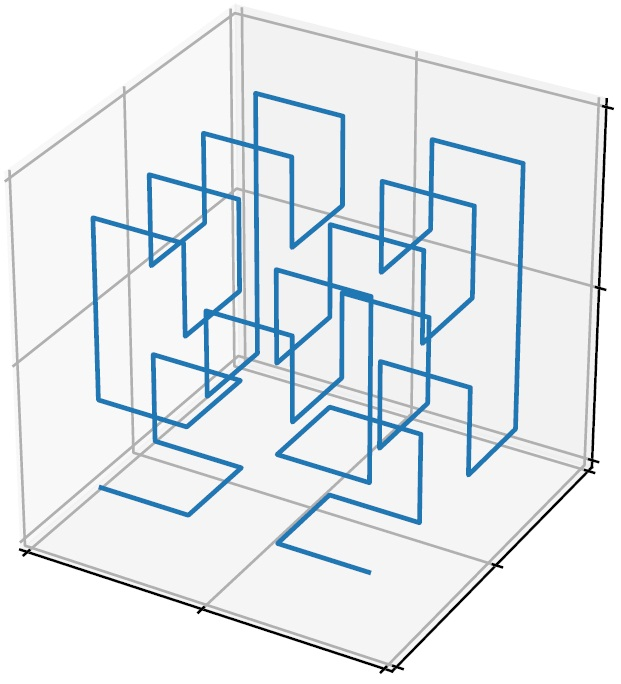
\includegraphics[width=0.9\linewidth]{fig1a.JPG} \\ (a)}
\end{minipage}
\begin{minipage}{0.45\linewidth}
\center{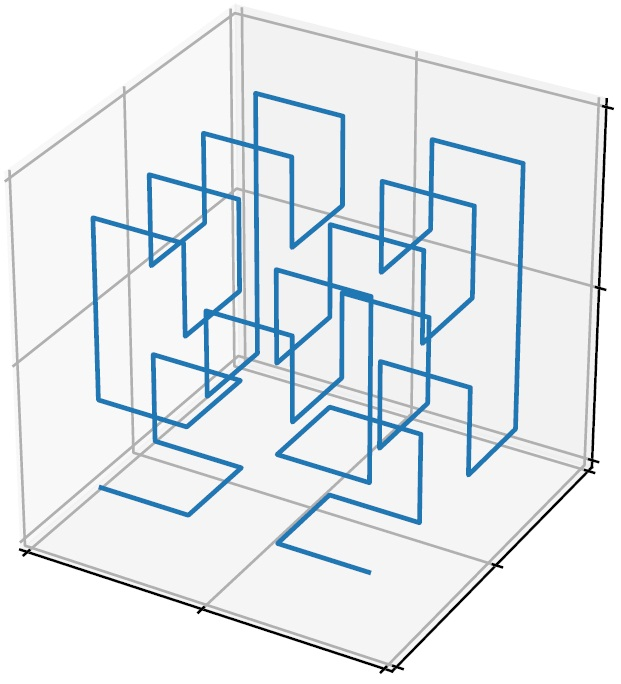
\includegraphics[width=0.9\linewidth]{fig1b.JPG} \\ (b)}
\end{minipage}
\caption{Evolvents with $m=4$ and (a) $N=2$, (b) $N=3$.}\label{fig:Peano}
\end{figure}   


Таким образом, в рамках данного подхода search trial в некотрой точке $x^k\in[0,1]$ будет включать в себя сначала the construction of the image $y^k=y(x^k)$, и лишь затем вычисление значения функции $ z^k = \phi(y^k)$.
Тройку значений $\{x^k,y^k,z^k\}$ мы будем называть outcome проведенного испытания.

%поправить название
\subsection{Асинхронный параллельный алгоритм поиска глобального минимума функции}

Используемый в данном исследовании параллельный алгоритм основан на информационно-статистическом подходе к разработке методов глобальной оптимизации, теоретические основы которого изложены в \cite{Strongin2000}. 

Нами была реализована асинхнонная схема распараллеливания вида ``master/worker''. В процессе-мастере выполняется алгоритм глобального поиска, в котором проводится накопление поисковой информации, оценка на ее основе константы Липшица для целевой функции, вычисление точек новых испытаний и распределение их по рабочим процессам. Процессы-рабочие получают от мастера точки, проводят в них новые испытания и отсылают мастеру результаты испытаний. 

Будем считать, что на каждой итерации процесс-мастер вычисляет одну точку нового испытания и передает ее для проведения испытания в процесс-рабочий. При этом проведение испытания рабочим является значительно более трудоемкой операцией, чем выбор новой точки мастером, что исключает простой процессов-рабочих. 
В данном случае (в отличие от синхронных параллельных алгоритмов) общее число выполненных испытаний каждым процессом-рабочим будет зависеть от трудоемкости проведения конкретного испытания и не может быть оценено заранее.

При описании параллельного алгоритма будем предполагать, что есть один процесс-мастер и $p$ рабочих процессов. Верхним индексом будем обозначать порядковый номер проведенного испытания, а нижний индекс будем использовать для нумерации испытаний в порядке возрастания координаты.
 
Начальная итерация проводится по особому правилу. Процесс-мастер (будем считать, что это процесс No 0) инициирует параллельное проведение $p$ испытаний в $p$ различных точках области поиска, две из которых являются граничными, а остальные --- произвольными внутренними точками (например, распределенными равномерно). Таким оборазом, начальные испытания проводятся в точках $\{y(x^1), y(x^2), ...,y(x^p)\}$, где $x^1 = 0$, $x^p = 1$, $x^i\in(0,1), i=2,..., p-1$.

Предположим теперь, что процессом-мастером получены результаты $k$ испытаний, и в текущий момент времени процессы-рабочие проводят испытания в точках $\{y(x^{k+1}), y(x^{k+2}), ...,y(x^{k+p})\}$. 

Пусть один из процессов (не ограничивая общности, можно считать, что это процесс No 1), в некоторый момент времени завершил проведение испытания в точке $y(x^{k+1})$.
Остальные процессы находятся в стадии проведения своих испытаний, т.е. в точках множества 
\[
I_k = \left\{ x^{k+2},...,x^{k+p} \right\}
\]
испытания уже начались, но еще не были завершены.

Тогда процесс No 1 пересылает процессу-мастеру полученные им результаты испытания, т.е. тройку  $\{x^{k+1},y^{k+1},z^{k+1}\}$.
Мастер сохраняет полученные результаты в своей информационной базе и выбирает для процесса No 1 точку нового испытания $x^{k+p+1}$ в соответствии с правилами, описанными ниже.

Step 1. Перенумеровать нижним идексом в порядке возрастания координаты точки множества
\[
X_k = \left\{x^1, x^2,...,x^{k+p} \right\},
\]
которое содержит все точки, в которых либо проведены, либо проводятся испытания, т.е.
\[
0=x_1<x_2<...<x_{x+p}=1.
\]
Step 2. Вычислить значения 
\[
M_1=\max \left\{ \frac{ \left|z_i - z_{i-1} \right|}{(x_i-x_{i-1})^{1/N}} : x_{i-1} \notin I_k, x_i \notin I_k, 2\leq i\leq k+p \right\},
\]
\[
M_2=\max \left\{ \frac{ \left|z_{i+1} - z_{i-1} \right|}{(x_{i+1}-x_{i-1})^{1/N}} : x_i \in I_k, 2\leq i < k+p \right\},
\]
\[
M=\max\{M_1,M_2\},
\]
где $z_i=\phi(y(x_i))$, if $x_i \notin I_k, \; 1\leq i \leq k+p$. Значения $z_i$ в точках $x_i \in I_k$ являются неопределенными, т.к. испытания в точках $x_i \in I_k$ еще не завершены. Если значение $M$ получилось равным 0, то присвоить $M=1$.

Step 3. Для каждого интервала $(x_{i-1},x_i), \; x_{i-1} \notin I_k, x_i \notin I_k, \; 2\leq i\leq k+p$, вычислить значение 
\[
R(i)=rM\Delta_i+\frac{(z_i-z_{i-1})^2}{rM\Delta_i}-2(z_i+z_{i-1}),
\]
называемое характеристикой данного интервала. Здесь $\Delta_i=\left(x_i-x_{i-1}\right)^{1/N}$, and $r>1$ is the reliability parameter of the method.

Step 4. Выбрать интервал $[x_{t-1},x_t]$ с наибольшим значением характеристики, т.е.
\[
R(t) = \max \left\{ R(i): \; x_{i-1} \notin I_k, x_i \notin I_k, \; 2\leq i\leq k+p \right\}.
\]

Step 5. Вычислить точку $x^{k+p+1} \in (x_{t-1},x_t)$ в соответствии с формулой
\[
x^{k+p+1} = \frac{x_{t}+x_{t-1}}{2} - \mathrm{sign}(z_{t}-z_{t-1})\frac{1}{2r}\left[\frac{\left|z_{t}-z_{t-1}\right|}{M}\right]^N.
\]

Сразу после вычисления точки $x^{k+p+1}$ очередного испытания процесс-мастер добавляет ее в множество $I_k$ и пересылает процессу-рабочему, который инициирует проведение испытания в ней. 

Процесс-мастер завершает работу алгоритма, если выполняется либо условие $\Delta_{t}<\varepsilon$ ($t$ --- номер интервала c максимальной характеристикой из Правила 4), либо условие $k>K_{max}$ ($k$ --- число выполненных испытаний).
Вещественное число $\varepsilon>0$ и целое число $K_{max}>0$ являются параметрами алгоритма и соответствуют точности поиска решения и максимальному числу испытаний.

Последовательный алгоритм глобального поиска, на основе которого была реализованна предложенный асинхронный алгоритм, допускает следующую интерпретацию \cite{Molinaro2001}. Используя точки ранее проведенных испытаний можно построить миноранту целевой функции, для которой значение $-R(i)$, где $R(i)$ --- значение характеристики интервала $(x_{i-1},x_i)$, будет являться значением миноранты в точке ее миинмума на интервале $(x_{i-1},x_i), 1\leq i\leq k+p$. В соответствии с правилом 4 алгоритма, новое испытание проводится в интервале с наименьшим значением миноранты. А в соответствии с правилом 5 точка нового испытания совпадает с точкой минимума миноранты.


%Нужен комментарий про практическую реализацию алгоритма - используемые технологии, основные моменты реализации и т.п.
%Асинхронный алгоритм глобального поиска был реализован с помощью технологии MPI, язык разработки --- С++.

Отметим, что описанная здесь асинхронная схема распалаллеливания в отличие от синхронных схем, использовавшихся ранее при решении ряда прикладных задач (see \cite{Kalyulin2017,Modorskii2016}), обеспечивает полную загрузку всех задействованных процессов при решении задач с разной трудоемкостью проведения испытаний в разных точках области поиска. Это подтверждается результатами экспериментов, описанными в следующем разделе.



%%%%%%%%%%%%%%%%%%%%%%%%%%%%%%%%%%%%%%%%%%
\section{Materials and Methods}


%%%%%%%%%%%%%%%%%%%%%%%%%%%%%%%%%%%%%%%%%%
\section{Results}

\subsection{Figures, Tables and Schemes}

All figures and tables should be cited in the main text as Figure~\ref{fig1}, Table~\ref{tab1}, Table~\ref{tab2}, etc.

\begin{figure}[H]

\includegraphics[width=10.5 cm]{Definitions/logo-mdpi}
\caption{This is a figure. Schemes follow the same formatting. If there are multiple panels, they should be listed as: (\textbf{a}) Description of what is contained in the first panel. (\textbf{b}) Description of what is contained in the second panel. Figures should be placed in the main text near to the first time they are cited. A caption on a single line should be centered.\label{fig1}}
\end{figure}   
\unskip

\begin{table}[H] 
\caption{This is a table caption. Tables should be placed in the main text near to the first time they are~cited.\label{tab1}}
\newcolumntype{C}{>{\centering\arraybackslash}X}
\begin{tabularx}{\textwidth}{CCC}
\toprule
\textbf{Title 1}	& \textbf{Title 2}	& \textbf{Title 3}\\
\midrule
Entry 1		& Data			& Data\\
Entry 2		& Data			& Data\\
\bottomrule
\end{tabularx}
\end{table}
\unskip

\begin{table}[H]
\caption{This is a wide table.\label{tab2}}
	\begin{adjustwidth}{-\extralength}{0cm}
		\newcolumntype{C}{>{\centering\arraybackslash}X}
		\begin{tabularx}{\fulllength}{CCCC}
			\toprule
			\textbf{Title 1}	& \textbf{Title 2}	& \textbf{Title 3}     & \textbf{Title 4}\\
			\midrule
			Entry 1		& Data			& Data			& Data\\
			Entry 2		& Data			& Data			& Data \textsuperscript{1}\\
			\bottomrule
		\end{tabularx}
	\end{adjustwidth}
	\noindent{\footnotesize{\textsuperscript{1} This is a table footnote.}}
\end{table}


\subsection{Formatting of Mathematical Components}

This is the example 1 of equation:
\begin{linenomath}
\begin{equation}
a = 1,
\end{equation}
\end{linenomath}
the text following an equation need not be a new paragraph. Please punctuate equations as regular text.
%% If the documentclass option "submit" is chosen, please insert a blank line before and after any math environment (equation and eqnarray environments). This ensures correct linenumbering. The blank line should be removed when the documentclass option is changed to "accept" because the text following an equation should not be a new paragraph.

This is the example 2 of equation:
\begin{adjustwidth}{-\extralength}{0cm}
\begin{equation}
a = b + c + d + e + f + g + h + i + j + k + l + m + n + o + p + q + r + s + t + u + v + w + x + y + z
\end{equation}
\end{adjustwidth}


% Example of a figure that spans the whole page width. The same concept works for tables, too.
\begin{figure}[H]
\begin{adjustwidth}{-\extralength}{0cm}
\centering

\includegraphics[width=13.5cm]{Definitions/logo-mdpi}
\end{adjustwidth}
\caption{This is a wide figure.\label{fig2}}
\end{figure}  

Please punctuate equations as regular text. Theorem-type environments (including propositions, lemmas, corollaries etc.) can be formatted as follows:
%% Example of a theorem:
\begin{Theorem}
Example text of a theorem.
\end{Theorem}

The text continues here. Proofs must be formatted as follows:

%% Example of a proof:
\begin{proof}[Proof of Theorem 1]
Text of the proof. Note that the phrase ``of Theorem 1'' is optional if it is clear which theorem is being referred to.
\end{proof}
The text continues here.

%%%%%%%%%%%%%%%%%%%%%%%%%%%%%%%%%%%%%%%%%%
\section{Discussion}

Authors should discuss the results and how they can be interpreted from the perspective of previous studies and of the working hypotheses. The findings and their implications should be discussed in the broadest context possible. Future research directions may also be highlighted.

%%%%%%%%%%%%%%%%%%%%%%%%%%%%%%%%%%%%%%%%%%
\section{Conclusions}

This section is not mandatory, but can be added to the manuscript if the discussion is unusually long or complex.

%%%%%%%%%%%%%%%%%%%%%%%%%%%%%%%%%%%%%%%%%%
%\section{Patents}

%This section is not mandatory, but may be added if there are patents resulting from the work reported in this manuscript.

%%%%%%%%%%%%%%%%%%%%%%%%%%%%%%%%%%%%%%%%%%
\vspace{6pt} 

%%%%%%%%%%%%%%%%%%%%%%%%%%%%%%%%%%%%%%%%%%
%% optional
%\supplementary{The following supporting information can be downloaded at:  \linksupplementary{s1}, Figure S1: title; Table S1: title; Video S1: title.}

% Only for the journal Methods and Protocols:
% If you wish to submit a video article, please do so with any other supplementary material.
% \supplementary{The following supporting information can be downloaded at: \linksupplementary{s1}, Figure S1: title; Table S1: title; Video S1: title. A supporting video article is available at doi: link.}

%%%%%%%%%%%%%%%%%%%%%%%%%%%%%%%%%%%%%%%%%%
\authorcontributions{For research articles with several authors, a short paragraph specifying their individual contributions must be provided. The following statements should be used ``Conceptualization, X.X. and Y.Y.; methodology, X.X.; software, X.X.; validation, X.X., Y.Y. and Z.Z.; formal analysis, X.X.; investigation, X.X.; resources, X.X.; data curation, X.X.; writing---original draft preparation, X.X.; writing---review and editing, X.X.; visualization, X.X.; supervision, X.X.; project administration, X.X.; funding acquisition, Y.Y. All authors have read and agreed to the published version of the manuscript.'', please turn to the  \href{http://img.mdpi.org/data/contributor-role-instruction.pdf}{CRediT taxonomy} for the term explanation. Authorship must be limited to those who have contributed substantially to the work~reported.}

\funding{Please add: ``This research received no external funding'' or ``This research was funded by NAME OF FUNDER grant number XXX.'' and  and ``The APC was funded by XXX''. Check carefully that the details given are accurate and use the standard spelling of funding agency names at \url{https://search.crossref.org/funding}, any errors may affect your future funding.}

\institutionalreview{Not applicable.}

\informedconsent{Not applicable.}

\dataavailability{In this section, please provide details regarding where data supporting reported results can be found, including links to publicly archived datasets analyzed or generated during the study. Please refer to suggested Data Availability Statements in section ``MDPI Research Data Policies'' at \url{https://www.mdpi.com/ethics}. If the study did not report any data, you might add ``Not applicable'' here.} 

%\acknowledgments{In this section you can acknowledge any support given which is not covered by the author contribution or funding sections. This may include administrative and technical support, or donations in kind (e.g., materials used for experiments).}

\conflictsofinterest{The authors declare no conflict of interest.} 

%%%%%%%%%%%%%%%%%%%%%%%%%%%%%%%%%%%%%%%%%%
%% Optional
\sampleavailability{Samples of the compounds ... are available from the authors.}

%% Only for journal Encyclopedia
%\entrylink{The Link to this entry published on the encyclopedia platform.}

%\abbreviations{Abbreviations}{
%The following abbreviations are used in this manuscript:\\
%
%\noindent 
%\begin{tabular}{@{}ll}
%MDPI & Multidisciplinary Digital Publishing Institute\\
%DOAJ & Directory of open access journals\\
%TLA & Three letter acronym\\
%LD & Linear dichroism
%\end{tabular}
%}

%%%%%%%%%%%%%%%%%%%%%%%%%%%%%%%%%%%%%%%%%%
%% Optional

%%%%%%%%%%%%%%%%%%%%%%%%%%%%%%%%%%%%%%%%%%
\begin{adjustwidth}{-\extralength}{0cm}
%\printendnotes[custom] % Un-comment to print a list of endnotes

\reftitle{References}

% Please provide either the correct journal abbreviation (e.g. according to the “List of Title Word Abbreviations” http://www.issn.org/services/online-services/access-to-the-ltwa/) or the full name of the journal.
% Citations and References in Supplementary files are permitted provided that they also appear in the reference list here. 

%=====================================
% References, variant A: external bibliography
%=====================================
\bibliography{bibliography}

%=====================================
% References, variant B: internal bibliography
%=====================================

% If authors have biography, please use the format below
%\section*{Short Biography of Authors}
%\bio
%{\raisebox{-0.35cm}{\includegraphics[width=3.5cm,height=5.3cm,clip,keepaspectratio]{Definitions/author1.pdf}}}
%{\textbf{Firstname Lastname} Biography of first author}
%
%\bio
%{\raisebox{-0.35cm}{\includegraphics[width=3.5cm,height=5.3cm,clip,keepaspectratio]{Definitions/author2.jpg}}}
%{\textbf{Firstname Lastname} Biography of second author}

% For the MDPI journals use author-date citation, please follow the formatting guidelines on http://www.mdpi.com/authors/references
% To cite two works by the same author: \citeauthor{ref-journal-1a} (\citeyear{ref-journal-1a}, \citeyear{ref-journal-1b}). This produces: Whittaker (1967, 1975)
% To cite two works by the same author with specific pages: \citeauthor{ref-journal-3a} (\citeyear{ref-journal-3a}, p. 328; \citeyear{ref-journal-3b}, p.475). This produces: Wong (1999, p. 328; 2000, p. 475)

%%%%%%%%%%%%%%%%%%%%%%%%%%%%%%%%%%%%%%%%%%
%% for journal Sci
%\reviewreports{\\
%Reviewer 1 comments and authors’ response\\
%Reviewer 2 comments and authors’ response\\
%Reviewer 3 comments and authors’ response
%}
%%%%%%%%%%%%%%%%%%%%%%%%%%%%%%%%%%%%%%%%%%
\end{adjustwidth}
\end{document}

